\chapter{Foundation - Technology Background}\label{chp:background}


%===================================================================================================%
\section{Introduction}
%===================================================================================================%

\blockquote{
    "Reviews of research literature are conducted for a variety of purposes. They include
    providing a theoretical background for subsequent research; learning the breadth of research on a
    topic of interest; or answering practical questions by understanding what existing research has to
    say on the matter. As such, research reviews are most often published as the introductory section
    of an article reporting a specific research study, or as one of the early sections of an academic
    thesis or dissertation. However, there exists another type of literature review that constitutes an
    original and valuable work of research in and of itself. Rather than providing a base for the
    researcher’s own endeavours, it creates a solid starting point for all other members of the
    academic community interested in a particular topic."\autocite{Okoli2010AResearch}
}

Based on this comprehensive and integrated understanding of research literature reviews and a systematic methodology which is defined in chapter~\vref{sec:LitRes}, this chapter introduces the necessary technology background as a foundation of common understanding for this research. Moreover, this section aims to provide the \textit{"solid starting point"} for all readers to engage with the topic. 

Seeing this study's research objective (chapter~\vref{chp:objective}) within the context of the scientific body of knowledge (chapter~\vref{chp:bodyOfKnow}), it becomes clear that it spans across four distinct domains of research: \textit{Internet of Things}, \textit{Event Stream Processing}, \textit{IoT Event Stream Processing} and \textit{Data Consumer Architecture Patterns}. Whereby \textit{IoT Event Stream Processing} is composed out of both \textit{Internet of Things} and \textit{Event Stream Processing} but shall be discussed as a distinct domain due to its importance for this study and its prominent placement in the title. 

Following an introduction of the system literature review method used in the subsequent sections, each of the four domains of research will be examined utilizing the review method defined earlier in order to ensure a systematic and reproducible research literature review. 

%===================================================================================================%
\section{Systematic Literature Review Method}\label{sec:LitRes}
%===================================================================================================%

The selection and review of research literature is a crucial step towards a holistic understanding of the current state of academic discussion. It is therefore utmost important to conduct it in a systematic and structured way to avoid misinformation or inchoate results. An early attempt to formalize research literature reviews was made by Fink in 2005:

\begin{displayquote}
    "[it is] a systematic, explicit,
    [comprehensive] and reproducible method for identifying, evaluating, and synthesizing
    the existing body of completed and recorded work produced by researchers, scholars, and
    practitioners."\autocite{Fink2015ConductingPaper}
\end{displayquote}

Since this approach is rather generic in order to fit many areas of research, Okoli and Schabram refined this methodology in 2010 and adapted it for \acf{IS} research. \\
According to Fink's definition, a proper and meticulous literature review is characterized by four important aspects. It should be \textit{systematic} in following a comprehensible methodological approach, \textit{explicit} in disclosing the way it was conducted, \textit{comprehensive} by including all relevant publications and therefore \textit{reproducible} and verifiable by others. 

\begin{figure}[ht]
    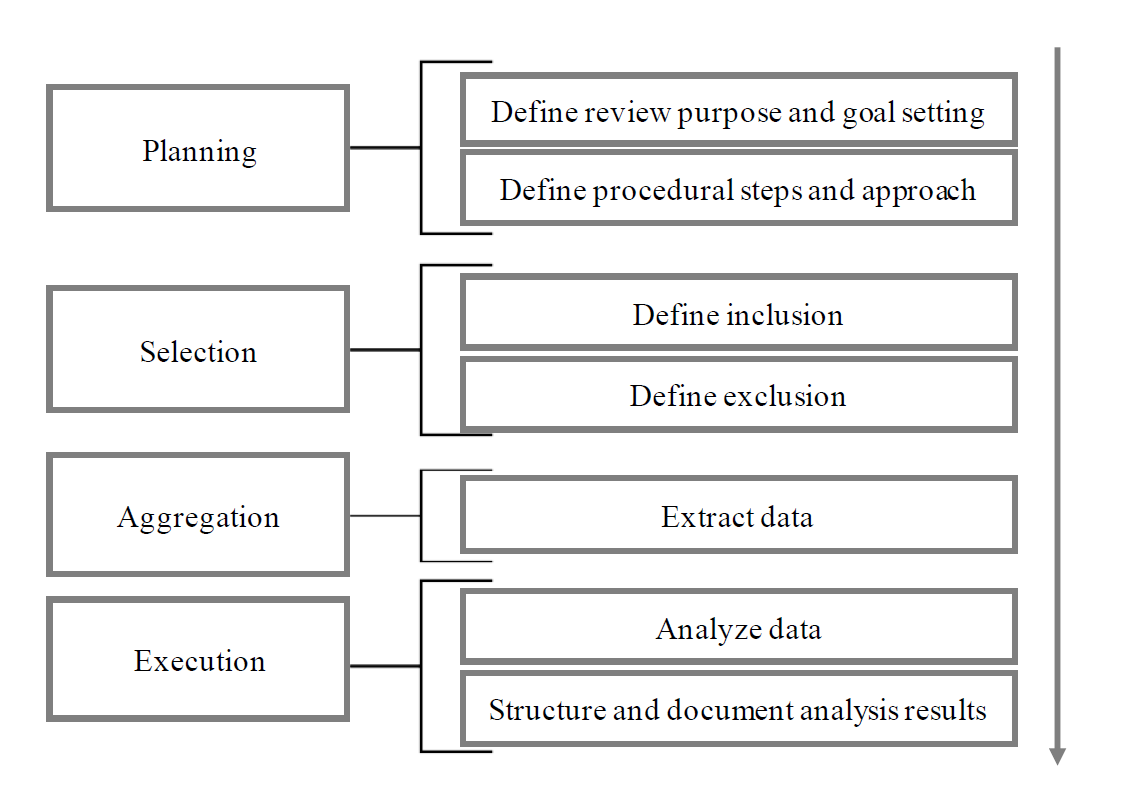
\includegraphics[width=0.8\linewidth]{images/methodology/litSearc.png}\centering
    \caption
    [Systematic Literature Review Method]
    {Systematic Literature Review Method (Source: \cite{Okoli2010AResearch})}
    \label{fig:litSearch}
\end{figure}

As depicted in Figure~\vref{fig:litSearch}, the Systematic Literature Review approach by Okoli and Schabram consists of 4 major steps: \\
\begin{enumerate}
    \item
    \textbf{Planning}\\
    First, the purpose of the research review and the goal has to be defined. This helps the reviewer to focus on research that is truly important for his or her academic paper and conduct a consistent and traceable review. Furthermore, procedural steps should be defined. One crucial part of the planning the choice of data source. To gather relevant research to review in the following steps, numerous search engines were used to accumulate enough source material for a sufficient literature review. The engines that were used are: 
    \begin{itemize}[nolistsep]
        \renewcommand\labelitemi{--}
        \item Google Scholar\footnote{\url{https://scholar.google.com}}
        \item Mendeley\footnote{\url{https://www.mendeley.com/research-papers/}}
        \item ScienceDirect\footnote{\url{https://www.sciencedirect.com/}}
        \item CiteSeerX\footnote{\url{http://citeseerx.ist.psu.edu/index}}
        \item Directory of Open Access Journals\footnote{\url{https://doaj.org}}
        \item IBM Northernlight (proprietary)\footnote{\url{https://ibm.northernlight.com/}}
    \end{itemize}
    All listed engines either inherently order by \textit{relevance} or provide the user with an option to do so. The algorithmic approach on how the relevance is calculated and assessed is assumed to be correct since it is not possible for the author to verify it within the scope of this research. Subsequently, the search results are reduced to the $20$ most relevant for each search engine in the first step. Secondly, duplicates are filtered and research that was erroneously included in the results (i.e., researches that belong to different domains) is removed. The remnant results are further selected, aggregated and analyzed.
    \item
    \textbf{Selection}\\
    In this step the inclusion and exclusion of research is defined and explained. The properties to decide on which paper is excluded or included must be clearly stated in order to \textit{explicitly} disclose the approach that was taken. In this paper, relevant articles were chosen by assessing the relevance of the research title and abstract. 
    \item
    \textbf{Aggregation}\\
    After the scientific body of knowledge assessed and parts of it selected in step $1$ and $2$, the information that is relevant for the paper on hand is extracted and aggregated. This step is mainly implicit because it is merely a reduction of the selected research to a applicable amount of excerpts to directly use in the paper and results in an implicit knowledge gained by the reviewer. It is possible that papers get rejected in this step due to the author assessing this research as not applicable for this study during the reading process.
    \item
    \textbf{Execution}\\
    The data is analyzed and results are presented to the reader. The main purpose of this step is to fulfill the goal defined in step $1$ and thus elevate the readers knowledge to a level that enables him or her to fully understand the authors research in the following chapters.
\end{enumerate}

The following sections will traverse these four steps in order to conduct a \textit{systematic} and \textit{consistent} research literature review. Some statements (especially step $1$ "Planning" and step $2$ "Selection") will be redundant for some domains but will be formulated nonetheless to \textit{explicitly} disclose how the results were achieved in order to maintain the \textit{reproducible} nature of this review.


%===================================================================================================%
\section{Internet of Things}
%===================================================================================================%

\begin{enumerate}
    \item
    \textbf{Planning}\\
    The purpose of this section is to give the reader a broad understanding of the industry and state of the academic research on this domain. It is not in scope to analyze different technical approaches and solutions for various use-cases but rather to enable the reader to understand the paper on hand by providing the necessary context and domain-specific terminology. Moreover, one major objective is to assess the importance of the domain and thus to confirm the significance and relevance of the research.\\
    Since the domain of \acf{IoT} is rather generic, the amount of results gathered from each search engine is expected to be vast.
    
    \item
    \textbf{Selection}\\
    For the search query \blockquote{Internet of Things}, the in Section~\vref{sec:LitRes} listed engines give the following numbers of results:
    
    \begin{itemize}[nolistsep]
        \renewcommand\labelitemi{--}
        \item Google Scholar: 2,930,000 results
        \item Mendeley: 39,826 results
        \item ScienceDirect: 58,532 results
        \item CiteSeerX: 282,506 results
        \item Directory of Open Access Journals: 1,425 results
        \item IBM Northernlight (proprietary): 21,070 results
    \end{itemize}
    
    Cumulated, the queries returned 3,333,359 results from which 140 where further examined. After filtering out duplicates, 82 papers remained. Likewise, 61 papers that were either to low-level technical or not fitting to the scope in another way were excluded from the literature review. The remaining 21 results propagated to the next step, the \textit{aggregation}.
    
    \item
    \textbf{Aggregation}\\
    The implicit aggregation of data sources resulted in a summary that can be read in the next section.
    
    \item
    \textbf{Execution}\\
    The term \ac{IoT} is more and more commonly used in academic publications, as well as non-academic media, whereby there is still no common definition. The \ac{IEEE} compiled an overview of different definitions of \ac{IoT} which will serve as a foundation basic foundation to design a comprehensive and inclusive definition for this study.\cfcite{Minerva2015TowardsIoT}
    
    A first attempt to define \ac{IoT} was made roughly 17 years ago by David L. Brock\cfcite{Brock2001TheObjects}.It focused on very basic, hardware-centric understandings of the term. 
    
    Other institutions, such as the \ac{ITU}, use a broader definition regarding the employed technologies as well as their usage:
    
    \begin{displayquote}
        "... global infrastructure for the Information Society, enabling advanced services
        by interconnecting (physical and virtual) things based on, existing and
        evolving, inter operable information and communication technologies."\autocite{Wortmann2015InternetThings}
    \end{displayquote}
    
    While according to the Cluster of European research projects on IoT
    
    \begin{displayquote}
        "The term "Things" is about active participants in different processes where
        they are able to communicate among themselves and the environment, by
        exchanging data and processing information sensed about the environment.
        They are able to react to world events and interact automatically with the
        environment by running programs that trigger actions with or without direct
        human intervention"\autocite{Gubbi2013InternetDirections}
    \end{displayquote}
    
    Another interesting take on the topic comes from Dorsemaine et. al.: 
    
    \begin{displayquote}
        "[...] ]a definition for
        a connected object could be: Sensor(s) and/or actuator(s) carrying
        out a specific function and that are able to communicate
        with other equipment. It is part of an infrastructure allowing
        the transport, storage, processing and access to the generated
        data by users or other systems.
        Then, a definition for the IoT would be: Group of infrastructures
        interconnecting connected objects and allowing
        their management, data mining and the access to the data they
        generate."\autocite{Dorsemaine2016InternetTaxonomy}
    \end{displayquote}
    
    As shown, there are several very broad definitions of the term \ac{IoT} that all try to avoid being too specific. Oriwoh et. al. addresses this problem and the purpose of any definition of the term:
    
    \begin{displayquote}
        "[...] the definition
        provided in this paper is only meant to serve as a guide to
        using the term and not as an absolute definition of what the
        term actually means. The description proposed in this work
        can be built upon as part of future research and development
        towards giving the term an even clearer meaning. In the
        meantime, its definition as ‘anything at all, depending on
        requirements’ suffices."\autocite{Oriwoh2015ThingsDefinition}
    \end{displayquote}
    
    
    This brings up an interesting point: the definition of a term, especially if the topic is as vague as the domain of \ac{IoT} is, should be tailored to the study's scope and requirements, since it only serves as a common foundation of understanding between author and reader to avoid any misunderstandings. With this in mind, this study defines \ac{IoT} as 
    
    \begin{displayquote}
        A great amount of uniquely identifiable devices that carry out a specific function and are able to communicate with other equipment. A vital part of the overall management structure is providing transport, storage and processing of sent messages to generate value. This function within the system is often carried out by an \ac{IoT} infrastructure management system. The system is able to react to events and interact automatically with system components that trigger actions with or without direct human intervention.
    \end{displayquote}
    
\end{enumerate}


%===================================================================================================%
\section{Event Stream Processing}
%===================================================================================================%

\begin{enumerate}
    \item
    \textbf{Planning}\\
    Similarly to the research review on \acf{IoT} research, the same seven search engines were used as a source. Likewise, the main goal is to give the reader a broad understanding of the domain and enables him to grasp the various concepts, patterns and practices in the realm of \acf{ESP}. Moreover, the purpose of this section is to explore the different limitations and challenges \acf{ESP} poses. Since it is the overall research objective to assess suitability and viability of serverless architectures for IoT Event Stream Processing, it is important to discuss and clarify the context in which the assessment will be conducted. 
    
    \item
    \textbf{Selection}\\
    For the search query \blockquote{Event Stream Processing} the following numbers of results were achieved:
    
    \begin{itemize}[nolistsep]
        \renewcommand\labelitemi{--}
        \item Google Scholar:  1,610,000 results
        \item Mendeley: 1,726 results
        \item ScienceDirect: 207,853 results
        \item CiteSeerX: 2,460,487 results
        \item Directory of Open Access Journals: 46 results
        \item IBM Northernlight (proprietary): 8,802  results
    \end{itemize}
    
    Cumulated, the queries returned 4,088,914 results from which 140 where further examined. After filtering out duplicates, 128 papers remained. Likewise, 113 papers that were either to low-level technical or not fitting to the scope in another way were excluded from the literature review. The remaining 15 results propagated to the next step, the \textit{aggregation}. In comparison to the selection process of IoT research, it is notable that only a fraction of the results were relevant or even related to the intended research domain.
    
    \item
    \textbf{Aggregation}\\
    The implicit aggregation of data sources resulted in a summary that can be read in the next section.
    
    \item
    \textbf{Execution}\\
    Event Stream Processing (or shorter \textit{Stream Processing} has become one of the most common computing tasks enterprise systems face today. As defined by the Gartner Research Institute,
    \blockquote{An event stream is a sequence of event objects arranged in some order, typically by time. \acf{ESP} is any kind of computing performed on event streams.}\autocite{Schulte2017TechnologyProcessing}\\
    In other words, \acf{ESP} processes data \textit{directly} as it is produced by nodes (i.e. applications, sensors, etc.). An "event" is often just defined as a "notable thing that happens".\autocite{Group2006Event-DrivenOverview} This is a very broad definition that has to be revised and adapted to the specific use-case at hand but none the less, a shared characteristic is that all events contain information, are generated as a byproduct of the occurrence of something and can be associated with a specific point in time. 
    Since many real world scenarios such as sensor measurements, financial trades, and so forth regularly result in a continuous stream of events, that \acf{ESP} is often a viable architectural approach.\\
    A common solution for this challenge is to store the data in a database and let applications query the data as needed or as scheduled. As depicted in~\vref{fig:dataRest}, the occurring events are sent from an application or sensor to an endpoint where they are stored at rest and the computation of said events has to be scheduled and managed. It is important to note that the information flow in this model centers around the data storage. First the information flows from the source to the storage and afterwards the downstream applications have to request it to access the information.
    
    \begin{figure}[ht]
        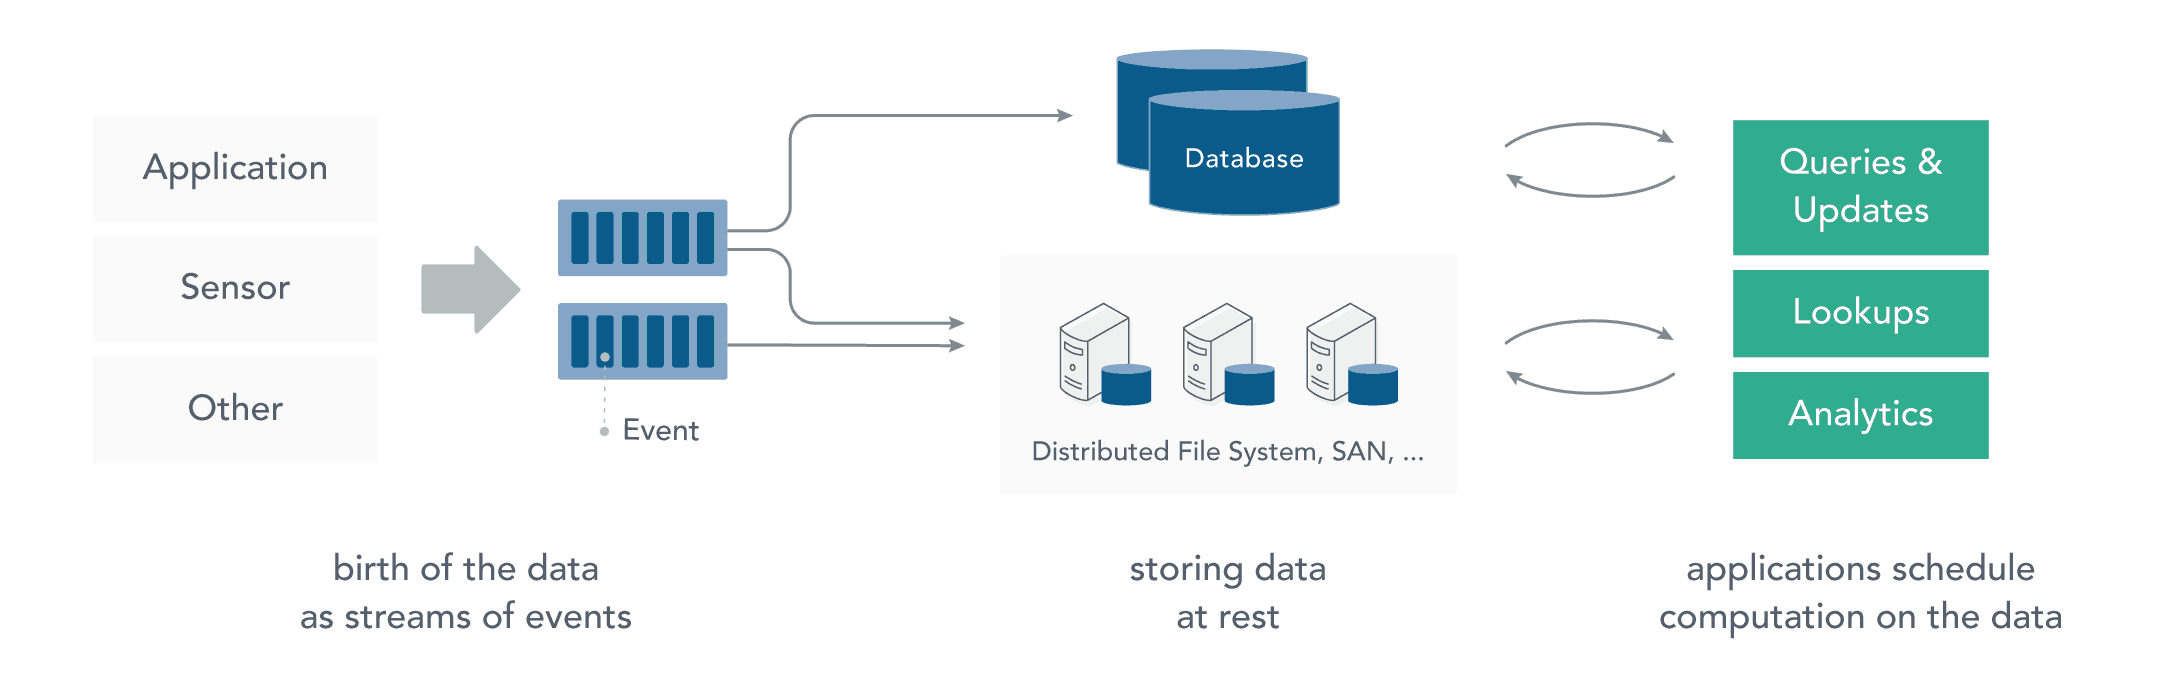
\includegraphics[width=\linewidth]{images/streaming/data_at_rest.png}\centering
        \caption
        [Data-at-Rest Architecture]
        {Data-at-Rest Architecture (Source: \cite{dataArtisans2017WhatProcessing})}
        \label{fig:dataRest}
    \end{figure}
    
    With Stream Processing however, a continuous data flow from left to right is established. Upon receiving an event from the stream, the \acf{ESP} application performs a task based on the event. For instance, this could be a transformation of the events' properties in order to match system-wide standards (e.g. unit conversation). 
    Figure~\vref{fig:dataStream} shows a simplified example of this pattern. Similarly to figure~\vref{fig:dataRest}, applications, sensors or other clients continuously generate events that are sent to an endpoint but instead of storing the data, it is directly processed by the assigned application. As indicated by the two arrows that lead from two streams to one single application, it is likewise possible to process multiple streams jointly and merge numerous information flows. The so-called \textit{stream processors} react directly upon receiving the events as mentioned before. 
    
    \begin{figure}[ht]
        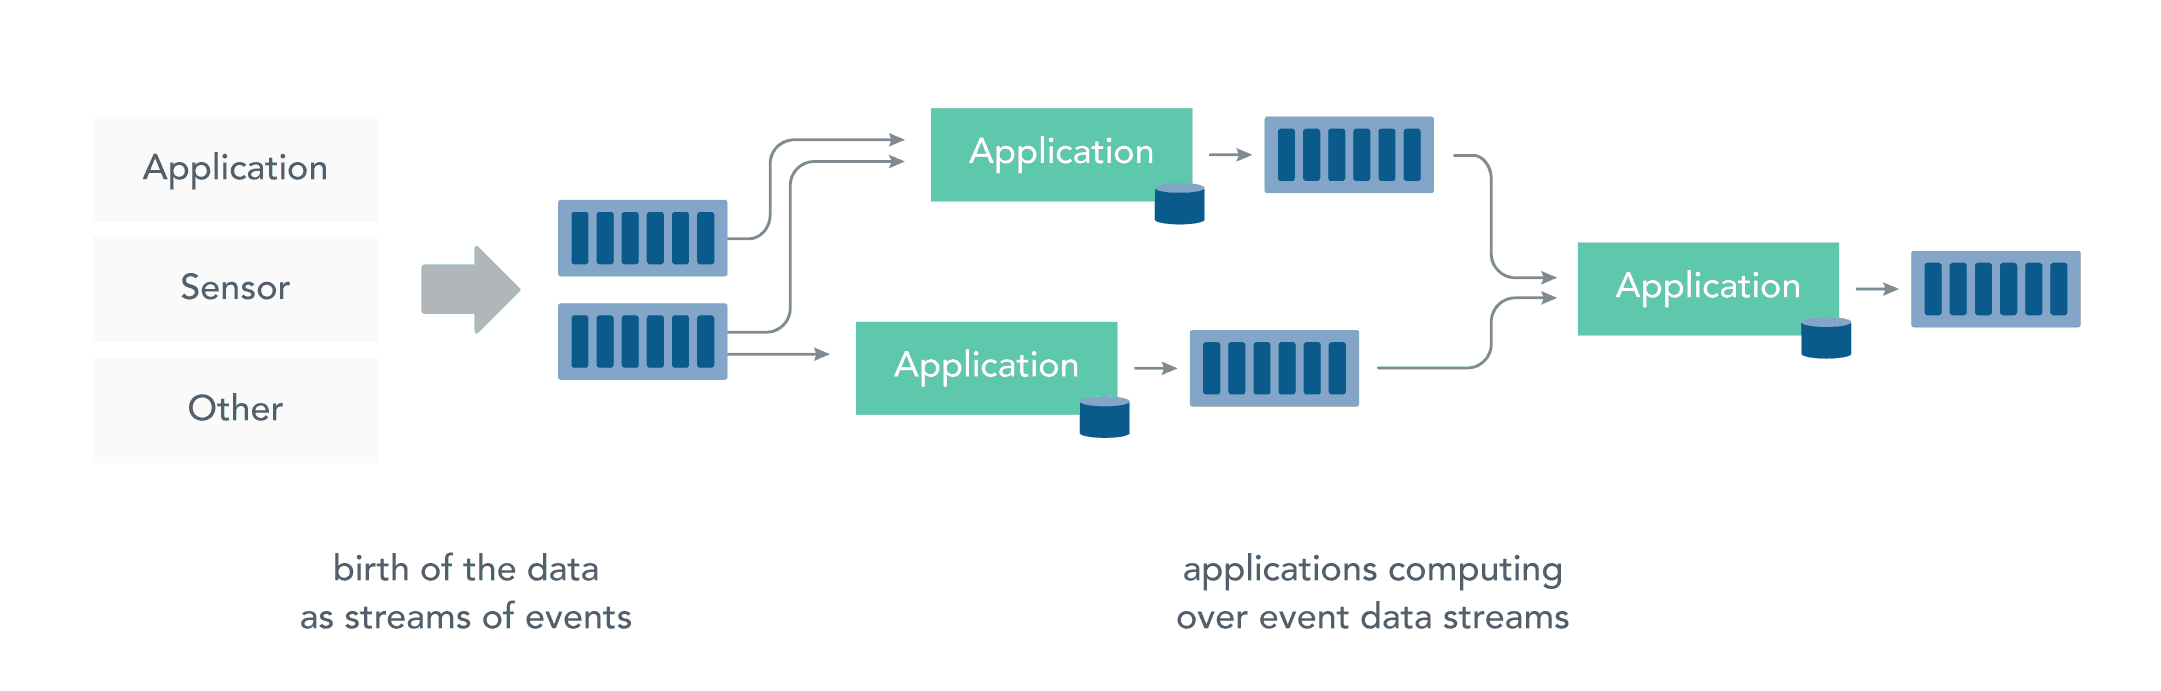
\includegraphics[width=\linewidth]{images/streaming/streming_data.png}\centering
        \caption
        [Stream Processing Architecture]
        {Stream Processing Architecture (Source: \cite{dataArtisans2017WhatProcessing})}
        \label{fig:dataStream}
    \end{figure}
    
    This seemingly minor change to the information flow has significant implications. To begin with, \acf{ESP} resembles the natural flow of data outside the IT system much closer than scheduled computation and is therefore easier to understand and design for. Secondly, since the event is processed immediately upon being received, the application can react instantly and a lag time between the occurrence of the event, the action trigger and the action itself can be avoided which results in a near real-time processing of information. 
    
    This approach allows for a data- and computation-driven perspective on complex business problems that aims to provide dynamic insights and need to handle a steady input of information. 
    Due to recent trends in the industry such as IoT and Industry 4.0, the amount of data that has to be processed, categorized and analyzed skyrocketed. The data-ingress often consists of semi-structured sets and has to be transformed and handled in near real-time.\autocite{Dekate2017PredictsInfrastructure} In order to provide valuable business insights for companies and public sector players alike, this approach is likely not only a temporarily trend but rather a long lasting evolution of how data-centric enterprise systems are being designed. Moreover, a recent Gartner report predicts that the market for \acf{ESP} solutions will grow by 15\% annually from 2017 to 2022 (compound annual growth rate).\autocite{Heudecker2017MarketProcessing} \\
    Many companies such as Netflix\footnote{\url{https://aws.amazon.com/solutions/case-studies/netflix-kinesis-streams/}} or Uber\footnote{\url{https://flink.apache.org/poweredby}} adopted stream-processing patterns in combination with serverless computing to take on challenges that demand highly scalable and performant systems. 
    This approach is particularly favourable for companies that deliver IoT solutions such as Toyota\footnote{\url{https://aws.amazon.com/solutions/case-studies/toyota-tsusho/}} or Quest\footnote{\url{https://customers.microsoft.com/en-us/story/quest}}.
    
\end{enumerate}


%===================================================================================================%
\section{IoT Event Stream Processing}
%===================================================================================================%

\begin{enumerate}
    \item
    \textbf{Planning}\\
    The background of this research is \blockquote{IoT Event Stream Processing}, hence the connection of both academic fields, IoT and Event Stream Processing, has to be discussed and put in context. Since the collection and selection of research has been done in the two previous sections it is not necessary to gather another sample of academic papers and hence the act of querying search engines can be omitted. Instead, papers from the preceding reviews that contain linking information for both IoT and ESP will be presented to connect both domains.
    
    \item
    \textbf{Selection}\\
    As mentioned above, this step has been already performed in the two previous sections
    
    \item
    \textbf{Aggregation}\\
    The implicit aggregation of data sources resulted in a summary that can be read in the next section.
    
    \item
    \textbf{Execution}\\
    Event Stream Processing approaches have become a key concept for deriving insights from the \ac{IoT} and have been recognized as pivotal building-blocks by both academia and industry. They provide a very well suited option for the increasing number of applications requiring such processing concepts. As discussed before, the \ac{IoT} creates a huge quantity of data that typically flows in streams in real-time. Generating value from this data-events largely depends on scalable stream-processing solutions that are able to adapt to changes and specific IoT settings.\cfcite{DeFrancisciMorales2016IoTMining}
    
    \begin{displayquote}
        "In the IoT data stream model, data arrives at high speed,
        and algorithms that process it must do so under very strict
        constraints of space and time. Consequently, data streams
        pose several challenges for data mining algorithm design.
        First, algorithms must work within limited resources (time
        and memory). Second, they must deal with data whose nature
        or distribution changes over time. We need to deal with
        resources in an efficient and low-cost way. In data stream
        mining, we are interested in three main dimensions:
        \begin{itemize}[nolistsep]
            \item accuracy
            \item amount of space (computer memory) necessary
            \item time required to learn from training examples and to predict
        \end{itemize}
        These dimensions are typically interdependent [...]"\autocite{DeFrancisciMorales2016IoTMining}
    \end{displayquote}
    
    The key takeaway from this excerpt is that IoT data stream models have to handle a remarkable amount of incoming data at high speed and must provide algorithms that process this data ingress in a timely manner. In addition, they must adapt to an ingress that changes its nature and distribution over time. 
    
    It is expected that the amount of connected devices sending messages will be around 20 to 50 million devices by 2020.\cfcite{2014TheThings}
    
    Naturally, each device will generate increasing amounts of data. Having the current tendency in mind, the transferred data over the internet is expected double its size every two years, reaching a total throughput of 44 Zettabytes, or 44 trillion Gigabytes by 2020.\cfcite{2014ExecutiveThings}
    
    With this amount of incoming data to process, it is evident that at some point the traditional strategy to store data-events before they are processed becomes too expensive and an event-driven stream-processing approach becomes more and more advantageously. This is the reason why the domain of IoT is such an obvious field to apply stream-processing.\cfcite{Soto2016CemlIoT}
    
    Khare et. al. give a very concise and comprehensive characterization of the intersection of IoT and Event Stream Processing:
    
    \begin{displayquote}
        "The Internet of Things (IoT) paradigm has given rise to
        a new class of applications wherein complex data analytics
        must be performed in real-time on large volumes of fastmoving
        and heterogeneous sensor-generated data. Such data
        streams are often unbounded and must be processed in a
        distributed and parallel manner to ensure timely processing
        and delivery to interested subscribers. Dataflow architectures
        based on event-based design have served well in
        such applications because events support asynchrony, loose
        coupling, and helps build resilient, responsive and scalable
        applications."\autocite{Khare2015ReactivePublish/subscribe}
    \end{displayquote}
    
    Especially the tendency of IoT systems to generate large sets of "fastmoving" data that have to be processed in real-time makes Event Stream Processing a predistined approach for many use-cases. These types of architectures have furthermore the inherent ability to handle asynchrone events in a very responsive and scalable manner, which makes them a very good fit.\\
    This consideration is supported by many others, including Akbar et. al.:
    
    \begin{displayquote}
        "Most of the IoT [generate] large data streams which have to be analyzed
        in near real-time. Solutions based on Complex Event Processing
        (CEP) have the potential to extract high-level knowledge from
        these data streams [...]"\autocite{Akbar2016Context-awareApplications}
    \end{displayquote}
    
    This shows that the intersection between IoT and Event Stream Processing is a very synergistic domain that holds interesting opportunities as well as challenges. The academic community \ac{ESP} architectures as a very suitable solution because of it's inherent features and nearly perfect fit. 
    
    To summarize, IoT Event Stream Processing is outlined by the following characteristics:
    
    \begin{itemize}[nolistsep]
        \item High amount of data
        \item Fastmoving arriving data 
        \item Incoming data that has to be processed in a very timely and efficient matter
        \item Streams have to adapt to changing ingress characteristics
        \item Streams have to process asynchronous data ingress
    \end{itemize}
    
    
\end{enumerate}


%===================================================================================================%
\section{Data Consumer Architecture Patterns}
%===================================================================================================%

\begin{enumerate}[label={}]
    \item
    \textbf{Planning}\\
    Since one major part of this study focuses on the processing of data within IoT Event Stream Processing architectures, this section is divided into containerized applications, which poses as the traditional alternative to serverless architectures, and serverless to have a more precise perspective on both topics that would be fuzzy when reviewing both topics at once.
    
    The purpose of this section is to give the reader a broad understanding of the industry and state of the academic research on the domain of data consumer architecture patterns. \\
    The selection, aggregation and execution of the literature review will be done in the to the domain corresponding subsections. 
    
    \item
    \textbf{Selection}\\
    The search query will be determined by the research domain in focus. The in Section~\vref{sec:LitRes} listed engines provide the foundation of academic publications to be aggregated and assessed. 
    
    \item
    \textbf{Aggregation}\\
    The implicit aggregation of data sources results in a summary that can be read in the following section.
    
    \item
    \textbf{Execution}\\
    The data is analyzed and results are presented to the reader. The main purpose of this step is to fulfill the goal defined in step $1$.
    
\end{enumerate}

%***************%
\subsection{Containerized Application}\label{chp:container}
%***************%


\begin{enumerate}
    \item
    \textbf{Selection}\\
    For the search query \blockquote{Containerized Application}, the in Section~\vref{sec:LitRes} listed engines give the following numbers of results:
    
    \begin{itemize}[nolistsep]
        \renewcommand\labelitemi{--}
        \item Google Scholar: 31,200 results
        \item Mendeley: 152 results
        \item ScienceDirect: 1,762 results
        \item CiteSeerX: 4,909 results
        \item Directory of Open Access Journals: 6 results
        \item IBM Northernlight (proprietary): 1,049 results
    \end{itemize}
    
    Cumulated, the queries returned 39,078 results from which 80 where further examined. After filtering out duplicates, 50 papers remained. Likewise, 40 papers that were either to low-level technical or not fitting to the scope in another way were excluded from the literature review. The remaining 10 results propagated to the next step, the \textit{aggregation}.
    
    \item
    \textbf{Aggregation}\\
    The implicit aggregation of data sources resulted in a summary that can be read in the next section.
    
    \item
    \textbf{Execution}\\
    
    Containerized applications are studied in a vast variety of academic and technological depth. Ranging from high-level business analysis, over architecture evaluation to hardware-related topics such as kernel semantics, it is necessary to narrow the scope of this literature review to a subset of the available literature that actively aids this study and provides insights that help the reader to understand the implications of this research.\\
    One vital step is therefore to find a common definition of the topic \textit{containerized applications}.
    
    \begin{displayquote}
        "[...] containerization does not execute a
        VM as a complete OS instance but runs as partial instances
        of the OS which reduces the CPU and memory overload and
        also provides the portability due to small size of containers.
        Unalike the existing
        virtualization approach, a containerization does not execute a
        VM as a complete OS instance but runs as partial instances
        of the OS which reduces the CPU and memory overload and
        also provides the portability due to small size of containers
        "\autocite{Kumar2017EconomicallyContainers}
    \end{displayquote}
       
    This means that containerized application have the benefit of being very small, compact and performant virtualized systems that are deployed on a running kernel to reduce CPU and memory overhead. It is not in scope of this study to fully discuss how virtualization on the level of the operating system works but to provide the reader with sufficient knowledge to understand the study, hence restraining from deeper literature study at this point. \\
    The key take-away is that containers provide a runtime for application that is very resource-preserving and portable. 
    
    There are different technologies available to implement container-based virtualization in a system. The most commonly used one according to "StackShare" is Docker by far.~\cfcite{2018DockerStackShare} Moreover, it is the only containerization technology used in the publications assessed in this literature review. In this study, Docker is therefore the only containerization technology in scope to avoid any misunderstandings. 
    
    
    
    
    
    \cfcite{Fink2014Docker:Framework}
    
    As a foundation for the literature review for the domain of containerized applications, the system characteristic matrix defined by Hammond and Rymer will be employed. It serves as a starting point for deeper examination of the different topics. 
    
    \begin{figure}[ht]
        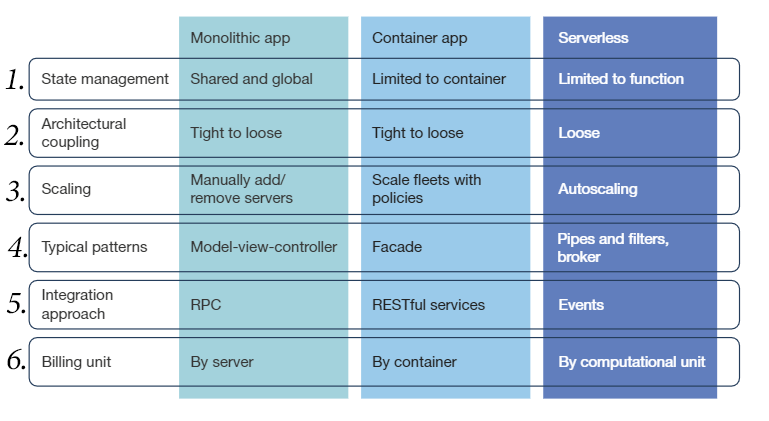
\includegraphics[width=\linewidth]{images/serverless/demyst2.png}\centering
        \caption
        ["Serverless" compared to traditional approaches]
        {"Serverless" compared to traditional approaches (Source: \cite{Hammond2018DemystifyingComputing})}
        \label{fig:slessCompared}
    \end{figure}
    
    \begin{enumerate}
        \item \textbf{State Management}\\
        is one of the areas where \textit{monolithic apps} have the most obvious advantage. The state is shared and global which reduces the required state management to a bare minimum.\\
        Since \textit{monolithic apps} are defined as one single system that offers many services using different interfaces that share the same global state.~\cfcite{Villamizar2015EvaluatingCloud} The management of this state is therefore not particularly complex and can be done inside of the system. For availability reasons, it might be a good idea to store the state redundantly but this is out of scope for the thesis and does not change the fact that the state of a \textit{monolithic app} is shared and global.
        
        \textit{Container Apps} on the other hand, have an inherent state management linked to the container instance. 
        
        \item \textbf{Architectural Coupling}
        
        \item \textbf{Scaling}
        
        \item \textbf{Typical Patterns}
        
        \item \textbf{Integration Approach}
        
        \item \textbf{Billing Unit}
    \end{enumerate}
    
       
    
    For a \textit{container app} on the other hand, state management is normally limited to the container. Since one of the main design principles of containerization is to confine the system within the boundaries of the container, it is possible to maintain a global shared state within the container itself but not to share it between all system services. If one container dies (e.g., reboot, failure, ...), it's state dies with it. Concepts like state-providers act as an external source of truth that can transfer and preserve state but often add complexity to the system and need to be implemented.~\cfcite{Ling2004SessionState}
    
    
\end{enumerate}
    

    
    


%***************%
\subsection{Serverless}\label{sec:serverless}\label{chp:serverless}
%***************%


\begin{enumerate}
    \item
    \textbf{Selection}\\
    For the search query \blockquote{Internet of Things}, the in Section~\vref{sec:LitRes} listed engines give the following numbers of results:
    
    \begin{itemize}[nolistsep]
        \renewcommand\labelitemi{--}
        \item Google Scholar: 12,700 results
        \item Mendeley: 157 results
        \item ScienceDirect: 79 results
        \item CiteSeerX: 1,320 results
        \item Directory of Open Access Journals: 0 results
        \item IBM Northernlight (proprietary): 683 results
    \end{itemize}
    
    Cumulated, the queries returned 14,939 results from which 100 where further examined. After filtering out duplicates, 40 papers remained. Likewise, 19 papers that were either to low-level technical or not fitting to the scope in another way were excluded from the literature review. The remaining 21 results propagated to the next step, the \textit{aggregation}.
    
    \item
    \textbf{Aggregation}\\
    The implicit aggregation of data sources resulted in a summary that can be read in the next section.
    
    \item
    \textbf{Execution}\\
    
    Similar to the literature review for containerized applications, the system characteristic matrix defined by Hammond and Rymer will be employed as a foundation for the literature review for the domain of serverless applications. Using the same matrix as a starting point ensures a basic comparability between both domain. It serves as a starting point for deeper examination of the different topics. 
    
        
    \begin{figure}[ht]
        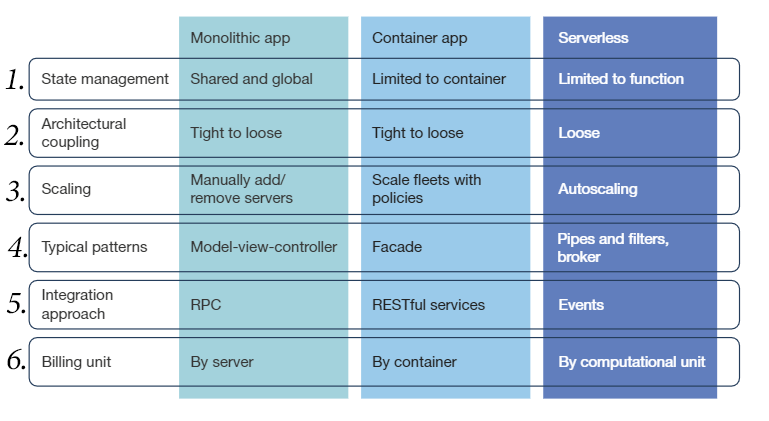
\includegraphics[width=\linewidth]{images/serverless/demyst2.png}\centering
        \caption
        ["Serverless" compared to traditional approaches]
        {"Serverless" compared to traditional approaches (Source: \cite{Hammond2018DemystifyingComputing})}
        \label{fig:slessComparedSl}
    \end{figure}
    
    \begin{enumerate}
        \item \textbf{State Management}\\
        Similarly, state management in \textit{serverless applications} can be complex due to the confined nature of its code. Since the application is spun up on invocation and only lives on for the computation time it is not possible to maintain state throughout different function invocations.
        
        \item \textbf{Architectural Coupling}
        
        \item \textbf{Scaling}
        
        \item \textbf{Typical Patterns}
        
        \item \textbf{Integration Approach}
        
        \item \textbf{Billing Unit}
    \end{enumerate}
    
    
    
    \begin{enumerate}\label{lst:serverlessCharacteristics}
        \item running back end code without managing your own server systems or your own server applications (containers or PaaS) $\longrightarrow$ no provisioning
        \item polyglot
        \item deployment is strange 
        \item completely automatic elastic scaling (provider regelt)
        \item multiple event types
        \item stateless
    \end{enumerate}
    \autocite{Roberts2016ServerlessArchitectures}
    
    "Serverless" is \textbf{the} new hype technology and is estimated to grow from USD 1.88 billion in 2016 to USD 7.72 billion by 2021, at a Compound Annual Growth Rate (CAGR) of 32.7\% according to "Markets and Research".\autocite{2017Function-as-a-Service2021} 
    
    Traditional approaches such as monolithic on-premise systems and even \acf{PaaS} based solutions or container clusters can be an option but have their own advantages and caveats. As shown in Figure~\vref{fig:slessCompared}, Hammond and Ryner identify six major categories to characterize architectural approaches.

    

    
    
    
    "Serverless" computing aims to solve those problems.\autocite{Roberts2016ServerlessArchitectures}

    
\end{enumerate}
    
%===================================================================================================%
\section{Summary}\label{chp:backgroundEND}
%===================================================================================================%